\chapter{Fixing ADD\_ADDR}
\label{chap:addaddr2}

\section{The ADD\_ADDR2 format}
There is an ongoing effort to move the current MPTCP specification \ref{6824} from Experimental to Standard Track. Solving the ADD\_ADDR vulnerability is believed to be a fundamental step to reach the required security standards for the transition to happen.
By analyzing the nature of the vulnerability, various proposals have been elaborated to modify the design of the ADD\_ADDR option [\rfc{7430}]. The conceptual flaw behind the option is that no secret material related to the ongoing MPTCP is included. The only security mechanism connected to such message is indeed the TCP-level sequence and acknowledge numbers, that an attacker has to know in order to inject such message into an ongoing session.
A possible solution could be to add the receiver token of the connection as a field in the ADD\_ADDR option. Such token, exchanged only during connection establishment via the MP\_CAPABLE option, is supposed to be unknown to the attacker that in turns would not be able to forge a valid ADD\_ADDR message. This solution wouldn't be effective if the attacker is able to eavesdrop the keys during the initial handshake; keys' eavesdrop is indeed a security concern related to MPTCP [ref to section on Keys' Eavesdrop], and for this reason it is not advisable to add such information in clear inside the ADD\_ADDR option, since that would give more opportunities for eavesdropping.
Another possibility would be to maintain the ADD\_ADDR format unchanged but to block the attack at a later stage. For example, if the destination address of the SYN packet is added as part of the message used to calculate the HMAC value, the attacker wouldn't be able to recompute the HMAC value after modifying the destination address. However, since addresses are not a stable piece of information in a network with NATs, using the destination address to calculate the HMAC might not work.
In order to achieve higher security levels maintaining NAT compatibility, a third option has been proposed with positive feedback. The idea is to add to the ADD\_ADDR option a new field containing the truncated HMAC value (rightmost 64 bits) calculated as follow: the \textit{key} is the MPTCP key of the sender as originally agreed in the MP\_CAPABLE handshake; the \textit{message} is the concatenation of the previous three fields in packet: Address ID, advertised IP address, and Port. The new format (figure \ref{fig:addaddr2} has been formally specified for the first time in \rfc{6824bis-04}.

\begin{figure}[!htb]
\centering
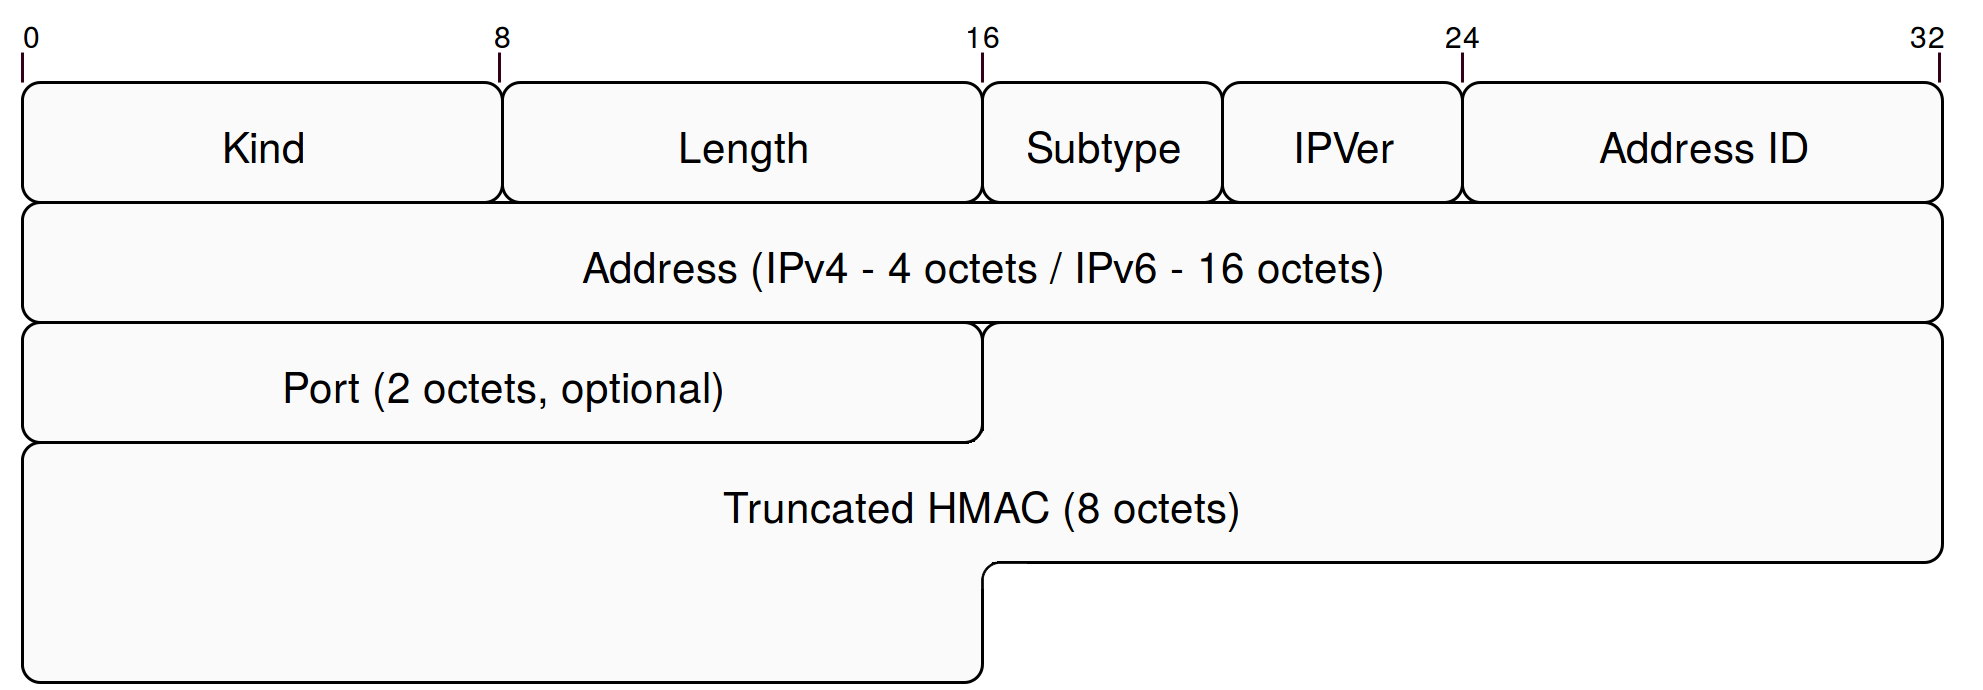
\includegraphics[width=0.75\textwidth]{images/addaddr2}
\caption{ADD\_ADDR2 option}
\label{fig:addaddr2}
\end{figure}

Such format would require the attacker to know the key in order to forge a valid ADD\_ADDR2 message, but such key is not exposed as in the case of the previous solution. Albeit, if the attacker is able to eavesdrop the keys during connection initiation it would be possible to exploit the same vulnerability even with the new address format. More experiments about this case are reported in section [ref to the experimental evaluation section]. Possible mitigations for such threat are explained in section [ref to keys' eavesdrop section 3.3.2].

The keys' eavesdrop threat is a partial-time on-path eavesdrop, a category that is considered less critical in terms of security concerns. Such keys' eavesdrop procedure in MPTCP has an almost identical counterpart in SCTP, when the SCTP-AUTH extension is used without pre-shared keys [\rfc{5061}]. In these regards the same security levels of SCTP would be reached in MPTCP by upgrading ADD\_ADDR to ADD\_ADDR2. Since SCTP is Standard Track, ADD\_ADDR2 is indeed considered a sufficient modification of the MPTCP first design to reach the security levels required for the transition to Standard Track.


\section{Implementing ADD\_ADDR2}
An introductory section that shows the main architectural aspects of how MPTCP has been merged into the TCP code and the TCP modules inside the kernel.
Here it starts the part with all the details about the implementation of ADD\_ADDR2 in the kernel, as part of the work developed during the stage. Code snippets have to be added here. The following subsections are the side issues and side features that have been elaborated during the thesis work.

\subsection{Retro-compatibility}
Version control mechanism was not present but it is needed to negotiate which format to use in a MPTCP session: ADD\_ADDR or ADD\_ADDR2.

\subsection{Port advertisement}
Port advertisement in ADD\_ADDR is possible according to RFC specifications but it was not part of the implementation at the beginning of the thesis work, so it has been added.

\subsection{IPv6 considerations}
Longer addresses brought some issues related to TCP option fields limitations.

\subsection{Crypto-API in MPTCP}
A major problem was how to deal with the new hashing requirements introduced by ADD\_ADDR2. Extending the current MPTCP hashing function to deal with input messages of arbitrary size is a first point to explain. The second part has to deal with the whole analysis related to adopting the kernel CRYPTO APIs to calculate the HMAC values in MPTCP and why this is not advisable.

\section{Other contributions}
Another minor part of the thesis work on MPTCP is related to some small contributions to the official RFC documentation and other open-source projects.

\section{Experimental evaluation}
This part should include performance analysis regarding the new format introduced with ADD\_ADDR2. A discussion on how the new format (and all the other modifications introduced with the patches) could impact any aspect of the protocol should be present in this section.
It is possible to add here the other possible solutions for ADD\_ADDR fix, and why they are not good enough. 